\documentclass{if-beamer}



% --------------------------------------------------- %
%                  Presentation info	              %
% --------------------------------------------------- %
\title[Projeto -- Apresentação final]{Arquitetura HIL para teste de sistemas embarcados como \textit{vehicle interface} de veículos autônomos baseados no Autoware}
\subtitle{Projeto -- Apresentação final}

\author[Gabriel Toffanetto]{\texorpdfstring
	{Gabriel Toffanetto França da Rocha 
		\\ \vspace{1mm} 
		\small{\href{mailto:g289320@dac.unicamp.br}{g289320@dac.unicamp.br}}
	}
	{Gabriel Toffanetto França da Rocha}
}

\institute[LMA/FEM/Unicamp]{\small{Professor Dr. Rodrigo Moreira Bacurau
  \\ \vspace{2mm}
  IM420X -- Projeto de Sistemas Embarcados de Tempo Real
  \\ \vspace{4mm}
  Faculdade de Engenharia Mecânica
  \\ \vspace{1mm}
  Universidade Estadual de Campinas}
}

\date{26 de novembro de 2024}

\logo{
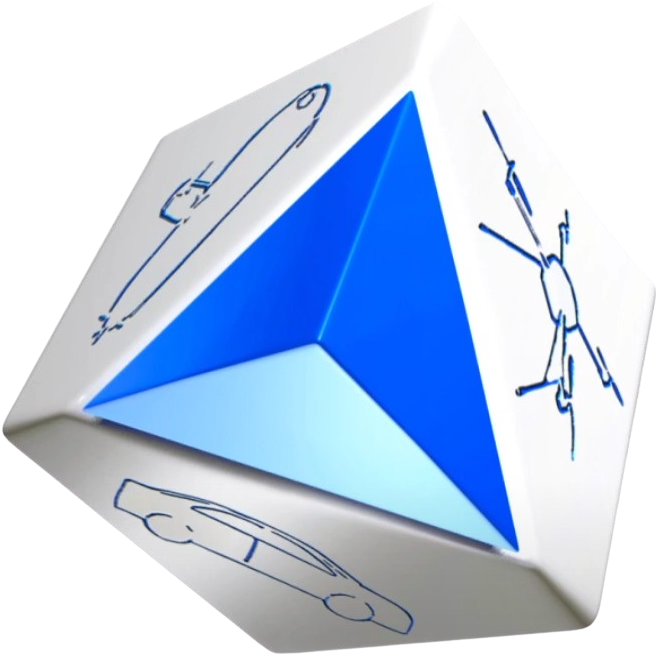
\includegraphics[width=1.2cm]{img/core/Logo_LMA_icon.png}
}


\subject{IM420X - Projeto final} % metadata

\graphicspath{{img/}}

\setbeamertemplate{caption}[numbered]

\newcolumntype{b}{>{\columncolor{white}}c}


\hypersetup{pdfpagemode=FullScreen}


% --------------------------------------------------- %
%                    Title + Schedule                 %
% --------------------------------------------------- %

\begin{document}

\begin{frame}
  \titlepage
\end{frame}

\begin{frame}{Agenda}
  \tableofcontents
\end{frame}

% --------------------------------------------------- %
%                      Presentation                   %
% --------------------------------------------------- %

\section{Introdução}


\section{Proposta}


\section{Sistema embarcado}

\subsection{\textit{Joystick}}

\begin{frame}{Processamento de sinais}
	
	\begin{columns}
		
		\begin{column}{0.5\textwidth}
			
			
			% TODO: \usepackage{graphicx} required
			\begin{figure}
				\centering
				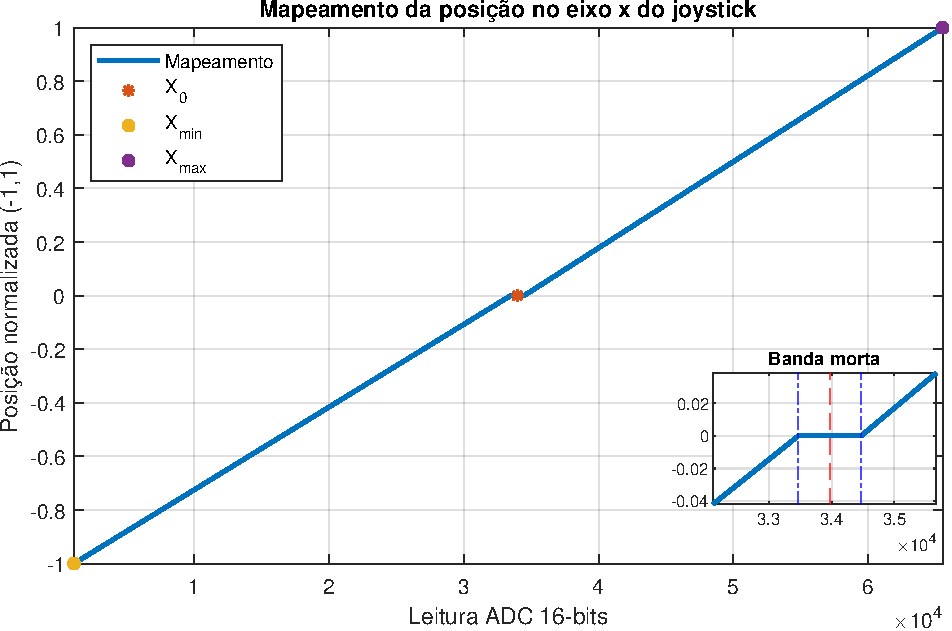
\includegraphics[width=1.1\linewidth]{plot_joy_x_axis.pdf}
				\caption{Mapeamento da posição normalizada do \textit{joystick} de acordo com a leitura analógia do ADC.}
				\label{fig:plotjoyxaxis}
			\end{figure}
			
		\end{column}
		
		\begin{column}{0.6\textwidth}
			
%if ((x(k) > (uiX0 + JOY_DEAD_BAND)) || (x(k) < (uiX0 - JOY_DEAD_BAND)))
%	if(x(k) - uiX0 > 0) 
%		X(k) = (x(k) - uiX0 - JOY_DEAD_BAND)/(uiXMax - uiX0 - JOY_DEAD_BAND); 
%	else
%		X(k) = (x(k) - uiX0 + JOY_DEAD_BAND)/(uiX0 - JOY_DEAD_BAND - uiXMin);
%else
%	X(k) = 0;
			
			\begin{equation}\label{eq:joy}
				p(v) = \begin{dcases}
					0\vphantom{\frac{0}{0}}, &\text{se } - B \le v - V_0 \le B \\
					\frac{v - V_0 - B}{V_{max} - V_0 - B}, &\text{se } v > V_0 + B \\
					\frac{v - V_0 + B}{V_0 - V_{min} - B}, &\text{se } v < V_0 - B 
				\end{dcases}
			\end{equation}
			
		\end{column}
		
	\end{columns}
	
\end{frame}


% -------------------------------------------------
%               Bibliografia.
%--------------------------------------------------
%\section{Referências bibliográficas}
%\begin{frame}{Referências bibliográficas}
%   %\bibliographystyle{acm}
%   \bibliography{bibliografia.bib}
%\end{frame}



\begin{frame}{}
	
	\begin{block}{}
		
		\centering
		\Huge{Obrigado!}
		
		\LARGE
		
		\vspace{5mm}
		
		Dúvidas?
		
	\end{block}
	
	\vspace{4mm}
	
	\begin{figure}[H]
		\centering
		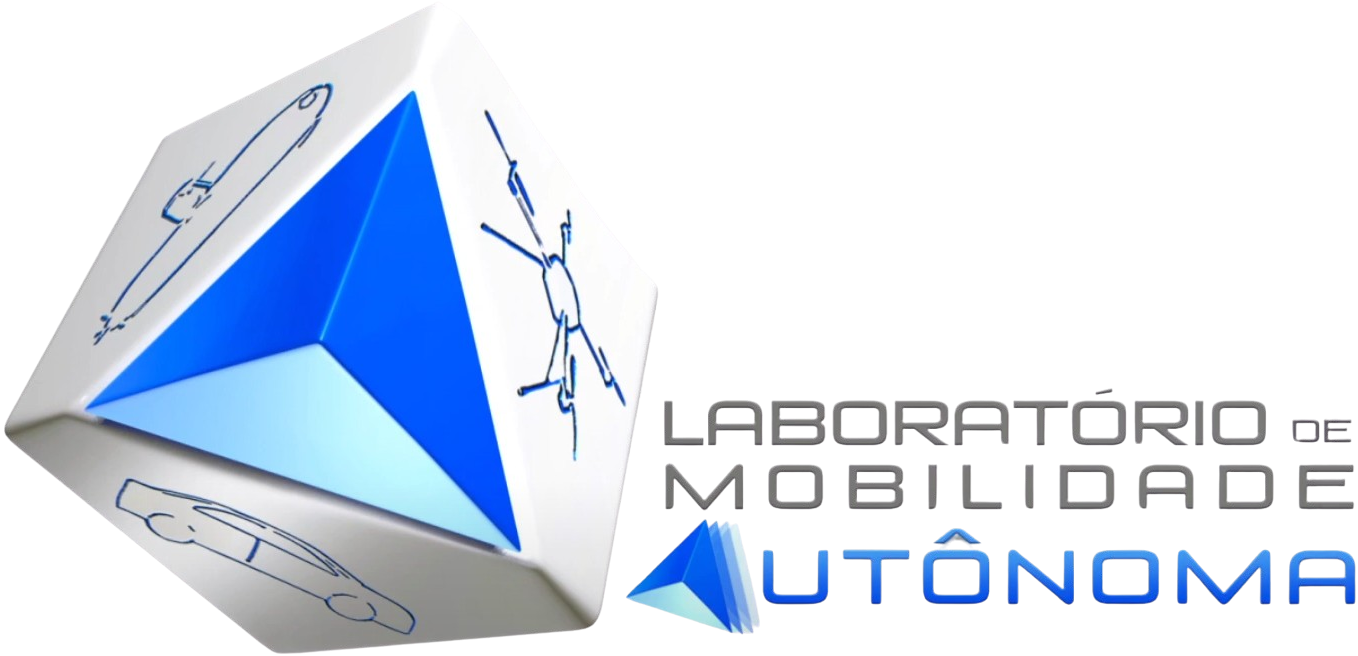
\includegraphics[width=0.5\linewidth]{img/core/Logo_LMA.png}
	\end{figure}
	
\end{frame}

\end{document}
